\documentclass[paper=a4,fontsize=10pt,DIV11,BCOR10mm]{scrartcl}


\usepackage[english]{babel}
\usepackage[utf8]{inputenc}
\usepackage[T1]{fontenc}
\usepackage{lmodern}

\usepackage{amssymb}
\usepackage{amsmath}
\usepackage{amsthm}
\usepackage{cancel}

\usepackage{graphicx}

\usepackage{url}
\usepackage{eurosym}


\usepackage{url}

\usepackage{placeins}

\newcommand{\abs}[1]{\left\lvert#1\right\rvert}
\newcommand{\norm}[1]{\left\lVert#1\right\rVert}
\DeclareMathOperator{\tr}{tr}




\titlehead{Technische Universität Berlin -- Fachgebiet Maschinelles Lernen\hfill \parbox[t]{2cm}{
\includegraphics[width=2cm]{../TU_Logo_kurz_RGB_rot}}}

\begin{document}

\title{Machine Learning I - Assignment 6\\
\small{Technische Universität Berlin}}


\author{\hspace{5cm}\textbf{Gruppe SciComp}\hspace{5cm} \and
	\small{Christoph Conrads (315565)} \and
	\small{Antje Relitz (327289)} \and
	\small{Benjamin Pietrowicz (332542)} \and
	\small{Mitja Richter (324680)}
}

\date{WS 2013/2014}

\maketitle


\section{Independence and Correlation}

I am renaming the variables from the exercise, since the used notation does not make sense to me.

Let $X\sim\mathcal{N}(0,1)$ and $Y=WX$, $P(W=1)=0.5, P(W=-1)=0.5$.

\subsection*{a)}
In the case of $W=1$ (or $P(W=1)=1$) we would get Y=X and therefore all the probability mass p(x,y) is on the diagonal y=x and the distribution of the mass on this line is just the same as for the density of the standardized Gaussian distribution.
\begin{figure}[htb]
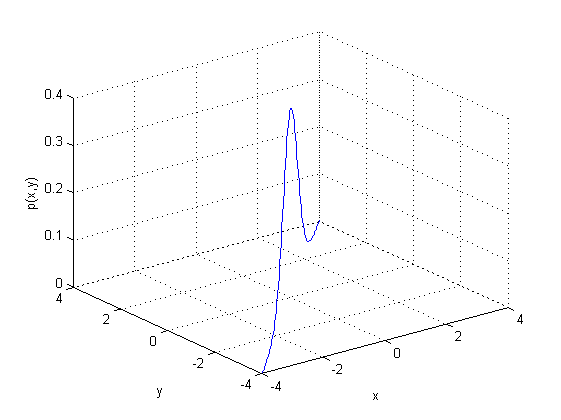
\includegraphics[scale=0.6]{prob_dist_wpos.png}
\caption{p(x,y) for W=1}
\end{figure}
\FloatBarrier

In the case of $W=-1$, all the probability mass would lie on the diagonal $y=-x$, the distribution on that line  would again look just like the density of the standardized Gaussian distribution.
\begin{figure}[htb]
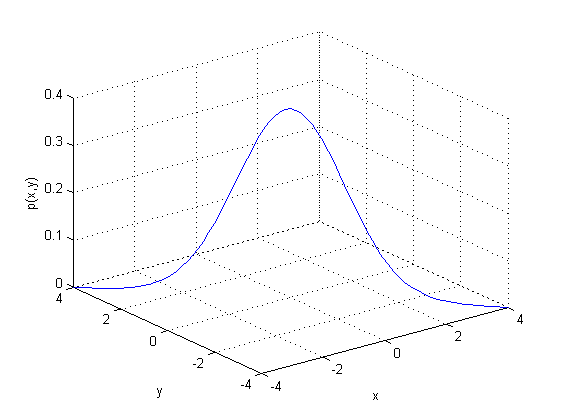
\includegraphics[scale=0.6]{prob_dist_wneg.png}
\caption{p(x,y) for W=-1}
\end{figure}
\FloatBarrier

For $Y=WX$ and $P(W=1)=0.5=P(W=-1)$ we just need to combine these two cases to get the joint density of $X$ and $Y$.
\begin{figure}[htb]
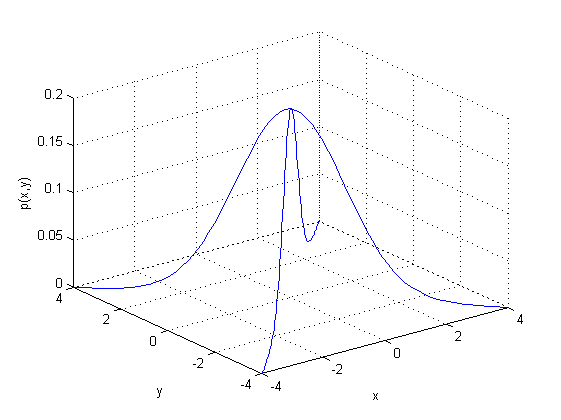
\includegraphics[scale=0.6]{prob_dist.png} 
\caption{Joint density function of x and y}
\end{figure}
\FloatBarrier

\subsection*{b)}
The density function of $X$ is given by $f_X(x)=\frac{1}{\sqrt{2 \pi}} e^{-\frac{1}{2}x^2}$ and the distribution function of $X$ is given by $F_X(x)=P(X\leq x)=\int\limits_{-\infty}^{x} \frac{1}{\sqrt{2 \pi}} e^{-\frac{1}{2}z^2}dz$.
Since $Y=WX$ we have:
\begin{align*}
F_Y(y)&=F_{WX}(y)=P(WX\leq y)\\
&= P(WX\leq y|W=1)\cdot P(W=1)+P(WX\leq y|W=-1)\cdot P(W=-1)\\
&= 0.5 \cdot P(X\leq y)+ 0.5 \cdot P(-X\leq y)\\
&= 0.5 \cdot P(X\leq y)+ 0.5 \cdot P(X \geq -y)\\
&= 0.5 \cdot \int\limits_{-\infty}^{y} \frac{1}{\sqrt{2 \pi}} e^{-\frac{1}{2}z^2}dz+ 0.5 \cdot \int\limits_{-y}^{\infty} \frac{1}{\sqrt{2 \pi}} e^{-\frac{1}{2}z^2}dz\\
\end{align*}
Since $\frac{1}{\sqrt{2 \pi}} e^{-\frac{1}{2}z^2}$ is symmetric with respect to the y-axis, we can change the integration boundaries in the second integral from $[-y,\infty)$ to $(-\infty,y]$, which yields:

\begin{align*}
F_Y(y)&= 0.5 \cdot \int\limits_{-\infty}^{y} \frac{1}{\sqrt{2 \pi}} e^{-\frac{1}{2}z^2}dz+ 0.5 \cdot \int\limits_{-\infty}^{y} \frac{1}{\sqrt{2 \pi}} e^{-\frac{1}{2}z^2}dz\\
F_Y(y)&= \int\limits_{-\infty}^{y} \frac{1}{\sqrt{2 \pi}} e^{-\frac{1}{2}z^2}dz
\end{align*}

This is the probability distribution function of a standardized normal distributed random variable and therefore $Y\sim\mathcal{N}(0,1)$.

\subsection*{c)}
We want to show $Cov(X,Y)=0$. We assume that $X$ and $W$ are independent and therefore $W$ and $X^2$ are independent and thus $\mathbb{E}[WX^2]=\mathbb{E}[W]\mathbb{E}[X^2]$. In addition we know that $\mathbb{E}[X^2]=Var(X)=1$ and $\mathbb{E}[W]=0$. We obtain
\begin{equation*}
Cov(X,Y)=\mathbb{E}[XY]=\mathbb{E}[WX^2]=\mathbb{E}[W]\mathbb{E}[X^2]=0\cdot 1=0
\end{equation*}
and therefore $X$ and $Y$ are uncorrelated.


\subsection*{d)}
We have to check, if $P(Y\leq y|X \leq x)=P(Y \leq y)$ holds for all $x$ and $y$. Since we want to construct a counter example, we can choose $x$ and $y$ arbitrarily and show that the equality does not hold. We know that $ P(Y \leq -1)<P(Y \leq 0)=0.5$ and therefore
\begin{equation*}
P(Y\leq -1|X \leq -1)=P(WX \leq -1|X\leq -1)=P(W=1)=0.5\neq P(Y \leq -1).
\end{equation*}
As a result, $X$ and $Y$ are not independent.



\section{Maximum Entropy Distribution}

\subsection*{a)}

Sei
\begin{flalign*}
	f(x) &= H(x) = -\int_{-\infty}^{+\infty} p(x) \log p(x) dx = -\int s(x) e^{s(x)} dx \\
	g_1(x) &= \mathbb{E}[x] = \int_{-\infty}^{+\infty} x p(x) dx = \int x e^{s(x)} dx = 0 \\
	g_2(x) &= \mathbb{E}[(x - \mathbb{E}[x])^2] - \sigma^2 = \int_{-\infty}^{+\infty} x^2 p(x) dx - \sigma^2 = 0 \\
\end{flalign*}
Dann ist das Maximierungsproblem
\[ \Lambda(s(x), \lambda_1, \lambda_2) = f(x) - \lambda_1 g_1(x) - \lambda_2 g_2(x) \]
Wir nehmen an, dass die Funktion $\log$ der Logarithmus zur Basis $e$ ist. Falls das nicht der Fall ist, muss die rechte Seite von $f$ mit dem Faktor $1 / \log(e)$ multipliziert werden. Ansonsten ändern sich die Ergebnisse aber nicht.



\subsection*{b)}

Wir berechnen das totale Differential nach $x$, um mögliche Lösungen für das Maximierungsproblem zu finden:
\[
	\frac{d\Lambda}{dx} = \frac{df}{dx} - \lambda_1 \frac{dg_1}{dx} - \lambda_2 \frac{dg_2}{dx}
	= -s(x) e^{s(x)} - \lambda_1 x e^{s(x)} - \lambda_2 x^2 e^{s(x)}
\]
Die notwendige Bedingung für ein Maximum ergibt folgendes:
\[ \frac{d\Lambda}{dx} = 0 = -s(x) \cancel{e^{s(x)}} - \lambda_1 x \cancel{e^{s(x)}} - \lambda_2 x^2 \cancel{e^{s(x)}} \Leftrightarrow s(x) = -\lambda_1 x - \lambda_2 x^2 \]
$s(x)$ ist potenziell quadratisch in $x$.
Wir betrachten die Berechnung des Erwartungswertes mit unserer Dichtefunktion:
\begin{flalign*}
	\mathbb{E}[x] &= \int_{-\infty}^{+\infty} x p(x) dx \\
	&= \int x e^{-\lambda_1 x - \lambda_2 x^2} dx \\
	&= \int_{-\infty}^0 x e^{-\lambda_1 x} e^{-\lambda_2 x^2} dx + \int_0^{+\infty} x e^{-\lambda_1 x} e^{-\lambda_2 x^2} dx \\
	&= 0
\end{flalign*}
Aufgrund des Erwartungswertes $\mathbb{E}[x] = 0$ müssen sich die Integrale links und rechts von $x = 0$ jeweils aufheben, also
\[ \int_{-\infty}^0 \abs{x} e^{-\lambda_1 x} e^{-\lambda_2 x^2} dx = \int_0^{+\infty} \abs{x} e^{-\lambda_1 x} e^{-\lambda_2 x^2} dx \]
Dabei fällt auf, dass $\abs{x}$ und $e^{-\lambda_2 x^2}$ symmetrische Funktionen sind, $e^{-\lambda_1 x}$ aber nur für $\lambda_1 = 0$. Also gilt
\[ s(x) = -\lambda_2 x^2 \]
und $s(x)$ ist quadratisch in $x$.



\subsection*{c)}

Weil $s(x)$ symmetrisch ist, ist $p(x)$ auch symmetrisch und damit gilt $\mathbb{E}[x] = 0$. Wir setzen
\[ \lambda_2 = \frac{1}{2 \sigma^2} \]
und ergänzen $p(x)$ um den Faktor $\sqrt{2 \pi \sigma^2}^{-1}$.



\subsection*{d)}

Wir wissen, dass $H(x)$ maximiert wird, wenn $x$ normalverteilt ist. Dann gilt $H(x^*) = H(x)$ und $J(x) = 0$. Weil $H(x^*)$ die Wert der Maximallösung ist, gilt für andere Verteilungen $x$ demnach $H(x^*) \geq H(x)$ und damit $J(x) \geq 0$.




\section{Approximations of Negentropy}

\subsection*{a)}

We define any quadratic function $G(y) = ay^2 + by + c$, with arbitrary constants $a,b,c \in \mathbb{R}$, take our assumption $E[y] = 0$ and begin to transform:

\begin{align}
E[G(y)] &= E[ay^2 + by + c] = aE[y^2] + b E[y] + c \stackrel{E[y] = 0}{=} aE[y^2] + c  \\
\text{Definition of Var: }Var[y] &= E[y^2] - E^2[y] \stackrel{E[y] = 0}{=} E[y^2] \\
\text{Using (2) in (1): } E[G(y)] &= aE[y^2] + c = aVar[y] + c
\end{align}

\subsection*{b)}
\begin{align*}
E[f(y)] = \int_{-\infty}^{\infty}f(y)p(y)\mathrm{d}y & \quad\quad
\frac{\partial E[f(y)]}{\partial y} = f(y)p(y)\\
p(y) \stackrel{E[y] = 0}{=} \frac{1}{\sqrt{2\pi}\sigma} exp{(-\frac{y^2}{2\sigma^2})} & \quad\quad p'(y) = - \frac{y}{\sqrt{2\pi}\sigma^3} exp{(-\frac{y^2}{2\sigma^2})}\\
\end{align*}

$max_y J(y) \implies \frac{\partial J(y)}{\partial y} \stackrel{!}{=} 0$
\begin{align*}
\frac{\partial J(y)}{\partial y} &= 2(E[G(y)]-E[G(\nu)]) \cdot G(y)p(y) \cdot \big(g(y)p(y) + G(y)p'(y)\big)\\
&= 2(E[ay^2 + by + c]-E[G(\nu)])\cdot (ay^2+by+c)p(y) \cdot \big((2ay+b)p(y) + (ay^2+by+c)p'(y)\big) \\
&\stackrel{E[y] = 0}{=} 2(aE[y^2] + c-E[G(\nu)])\cdot (ay^2+by+c)p(y) \cdot \big((2ay+b)p(y) + (ay^2+by+c)p'(y)\big) \\
&= 2(aE[y^2] + c-E[G(\nu)])\cdot \big((ay^2+by+c)(2ay+b)p^2(y) + (ay^2+by+c)(ay^2+by+c)p'(y)p(y) \big) \\
\end{align*}

\subsection*{c)}
\begin{align*}
J(w) &= (E[G(w^Tx)] - E[G(\nu)])^2 \\
\frac{\partial J}{\partial w} &= 2(E[G(w^Tx)] - E[G(\nu)]) \cdot G(w^Tx)p(w^Tx) \cdot \big( xg(w^Tx) p(w^Tx) + xG(w^Tx)p'(w^Tx)\big)
\end{align*}

\subsection*{d)}
\begin{align*}
\frac{\partial J}{\partial w} =& 2(E[G(w^Tx)] - E[G(\nu)]) \cdot G(w^Tx)p(w^Tx) \cdot \big( xg(w^Tx) p(w^Tx) + xG(w^Tx)p'(w^Tx)\big) \\
=& 2(E[a(w^Tx)(w^Tx)^T + b(w^Tx) + c] - E[G(\nu)]) \cdot (a(w^Tx)(w^Tx)^T + b(w^Tx) + c)p(w^Tx)\\&
 \cdot \bigg( x\big(2a(w^Tx)x + bx\big) p(w^Tx) + x(a(w^Tx)(w^Tx)^T + b(w^Tx) + c)p'(w^Tx)\bigg) \\
=& 2(aE[w^Txx^Tw] + bE[w^Tx] + c - E[G(\nu)]) \cdot (a(w^Tx)(w^Tx)^T + b(w^Tx) + c)p(w^Tx)\\&
 \cdot \bigg( x\big(2a(w^Tx)x + bx\big) p(w^Tx) + x(a(w^Tx)(w^Tx)^T + b(w^Tx) + c)p'(w^Tx)\bigg) \\
\end{align*}



%\begin{thebibliograpy}
%	\bibitem{DHS2000} R. O. Duda, P. E. Hart and D. G. Stork. \emph{Pattern Classification}. 2nd ed. New York, NY, USA: Wiley-Interscience, 2000. ISBN: 0-4710-5669-3
%\end{thebibliograpy}

\end{document}
